%  Copyright (C) 2002 Regents of the University of Michigan, portions used with permission 
%  For more information, see http://csem.engin.umich.edu/tools/swmf

\section{Appendix A: The Fermi function calculation approach}

For $g_e\ge1,\,\nu>-1$ the Fermi function may be developed into
convergent power series (see Eq.(5) from \cite{mcleod}):
\begin{equation}
{\rm Fe}_\nu(g_e)=\sum_{n=1}^\infty{\frac{(-1)^{n+1}}{n^{\nu+1}(g_e)^n}}.
\end{equation} 

The Taylor series in powers of $-\log(g_e)$ (see Eq.(6) from \cite{mcleod}): % from MacLeod
\begin{equation}
{\rm Fe}_{\nu}(g_e) = \sum_{i=0}^\infty{\frac{(1-2^{i-\nu}) \zeta(\nu+1-i)}{i!} (-\log(g_e))^i}.
\end{equation}
is only used for $g_e \in [e^{-3}; 1)$, because it converges when $|\log(g_e)| < \pi$.

For $0 < g_e < e^{-3}$ we use the following asymptotic series (see Eq.(8) from \cite{mcleod}): % from MacLeod
\begin{equation}
{\rm Fe}_{\nu}(g_e) \sim \frac{(-\log(g_e))^{\nu+1}}{\Gamma(k+2)} \left(1 + \sum_{i=1}^\infty{a_{2i} (\log(g_e))^{-2i}}\right).
\end{equation}
where
\begin{equation}
a_{2i} = \frac{(1 - 2^{1-2i})(k+1)!(2\pi)^{2i}}{(k+1-2i)!} \frac{|B_{2i}|}{(2i)!}.
\end{equation}
where $B_j$ denotes a standard Bernoulli number. The last formula can be simplified using the following expression for the Bernoulli numbers (see Eq.(9.616) from \cite{gradshtein}):
\begin{equation}
B_{2i} = \frac{(-1)^{i-1} (2i)!}{2^{2i-1} \pi^{2i}} \zeta(2i).
\end{equation}
so that
\begin{equation}
a_{2i} = \frac{2 (1 - 2^{1-2i}) (k+1)!}{(k+1-2i)!} |\zeta(2i)|.
\end{equation}

We only calculate the first three sum terms of the asymptotic series to get the best
approximation of ${\rm Fe}_\nu(g_e)$ for $g_e$ around $e^{-3}$:
\begin{equation}
{\rm Fe}_\nu(g_e) \approx \frac{(-\log(g_e))^{\nu+1}}{\Gamma(k+2)} \left(1 + \frac{a_2}{(\log(g_e))^2} + \frac{a_4}{(\log(g_e))^4}\right).
\end{equation}
An  asymptotic series does not guarantee an improvement in accuracy while increasing the number of the sum terms
involved. In our particular case the use of either more than or less than three sum
terms noticeably lowers the accuracy of ${\rm Fe}_\nu(g_e)$ for $g_e \in [e^{-5}, e^{-3}]$.

In both series $\zeta(x)$ denotes the Riemann zeta-function.
At $x > 0$ it can be calculated as a convergent series (see Eq.(9.522.2) from \cite{gradshtein}): % Gradshtein, Ryzhik: 9.522.2; Abramowitz: 23.2.19
\begin{equation}
\zeta(x) = \frac{1}{1-2^{1-x}} \sum_{n=1}^\infty{(-1)^{n+1} \frac{1}{n^x}}.
\end{equation}
At $x < 0$ we use the following reflection formula (see Eq.(7) from \cite{mcleod}): % MacLeod
\begin{equation}
\zeta(x) = 2^x \pi^{x-1} \sin(\frac{\pi x}{2}) \Gamma(1-x) \zeta(1-x).
\end{equation}

\begin{figure}[ht]
\centering
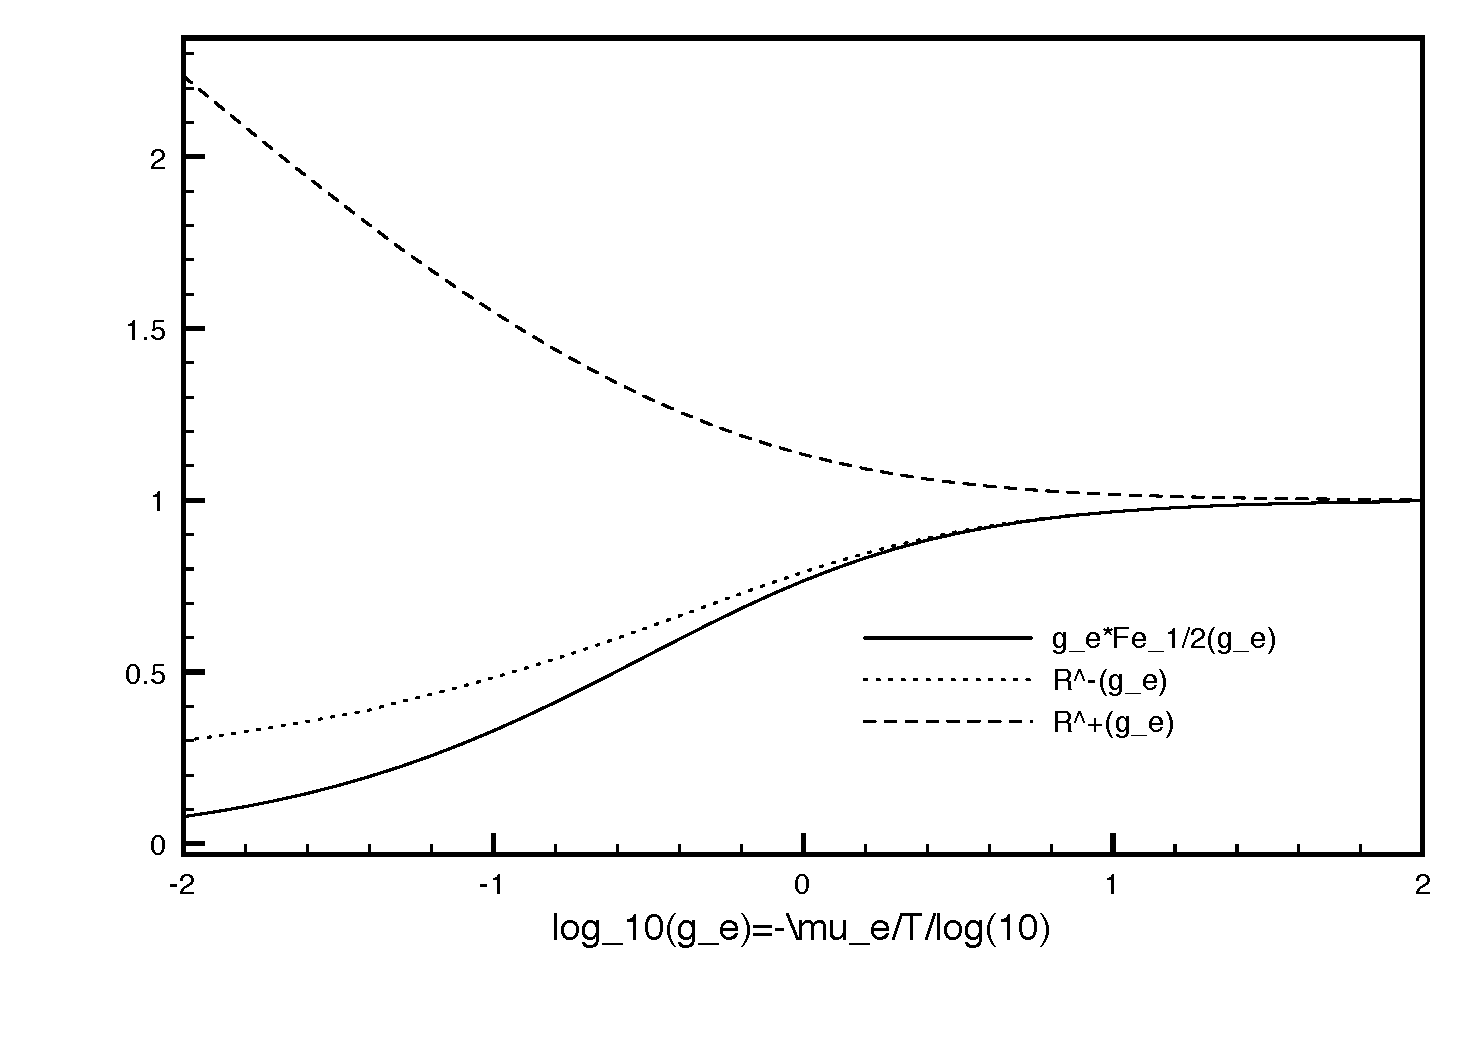
\includegraphics[scale=0.6]{FermiFunction.eps}
\caption{The Fermi function of index 1/2 multiplied by $g_e$ (solid) and the ratio functions (dashed) calculated using the described algorithm.}
\end{figure}

